\section{Experiments}
\label{sec:Experiments}
In this section, we discuss and compare the performance of MALTS with other competing methods on a few different simulation setups with continuous covariates, discrete covariates and mixed (continuous+discrete) covariates. Lastly, we demonstrate MALTS performance for estimating ATE on LaLonde's NSW and PSID-2 data samples \citep{lalonde}. 

MALTS performs an $\eta$-fold honest causal inference procedure. We execute a stratified splitting of the observed samples $\mathcal{S}_n$ into $\eta$ equal parts such that each part has similar ratio of treated to control units. For each fold, we use one of the $\eta$ partitions as training set $\mathcal{S}_{tr}$ (not used for matching) and rest of the $\eta-1$ partitions as the estimation set $\mathcal{S}_{est}$. 
%We repeat the training and estimation procedure $\eta$ times, once for each partition as a training set. 
% As the $\eta$-fold MALTS repeats the training and estimation procedure $\eta$ times, such that each fold uses a different partition of the observed sample $\mathcal{S}_n$, we have $\eta$ estimates of $\mathcal{M}$ (one for each of the $\eta$ folds), $\eta-1$ estimates of CATEs and $\eta-1$ matched groups for each unit. 
Using the output from each of the $\eta$-folds, we calculate the average estimated CATE for each unit, average estimated distance metric and a weighted unified matched group for each unit $s_i \in \mathcal{S}_n$. The weight of each matched unit $s_k$ corresponds to the number of times a particular unit $s_k$ was in the matched group of unit $s_i$ across the $\eta-1$ constructed matched groups. Here, $\eta$ was chosen to be 5 in our experiments. 

For interpretability, we let $\mathcal{M}_c$ be a diagonal matrix, which allows stretches of the continuous covariates. (Note that $\mathcal{M}_d$ is always diagonal.) This way, the magnitude of an entry in $\mathcal{M}_c$ or $\mathcal{M}_d$ provides the relative importance of the indicated covariate for the causal inference problem.

We further analyzed strategies for variance estimation for MALTS, performance under limited overlap between the covariates distribution of treated and control groups, and sensitivity to unobserved confounding shown in Appendix~B. 

%For all the experiments in this section, we use 5-fold MALTS i.e., we split the dataset into 5 equal parts using stratified sampling, and for each fold we use one of them as a training set (different one each for each fold) and other four as estimation set.

\subsection{Data Generative Processes}
In this subsection we describe the data generation process used in the simulation experiments. We use two main data-generative processes: The first DGP has a linear baseline with linear and quadratic treatment effects while the second DGP is the extension of Friedman's function introduced to test performance of prediction algorithms of \cite{friedman1991multivariate}. This second DGP, also termed as Friedman's DGP, has a scaled cosinusoidal treatment effect.
\subsubsection{Quadratic DGP} \label{dgp1}
This simulation includes both linear and quadratic terms.
% The quadratic simulation setup has a linear baseline, a linear treatment effect and a quadratic treatment effect term with interactions across important covariates.
Let $\mathbf{x}_{i,p}$ be a $p$-dimensional covariate vector composed of $p_c$ continuous covariates and $p_d$ discrete ones.
% where the first $p_c$-dimensions are drawn from a continuous distribution and the next $p_d$-dimensions are drawn from a discrete distribution. 
% The first $k_c$ dimensions of the continuous part of the vector and the first $k_d$ dimensions of the discrete part of the vector contribute to outcome determination. 
There are $k = k_{c} + k_{d}$  relevant covariates and the rest of the dimensions are irrelevant. As a shorthand, $p_c,k_c,p_d,$ and $k_d$ refer to the the subsets of indices of the covariates: all continuous, relevant continuous, all discrete, and relevant discrete, respectively.
% we represent $p_c$ as the set of indices for the continuous covariates, $p_d$ as the set of indices for the discrete covariates, $k_c$ as the set of indices for the relevant continuous covariates and $k_d$ as the set of indices for the relevant discrete covariates.
$\mathbf{x}_{i,k_c}$ and $\mathbf{x}_{i,k_d}$ refer to the vectors of relevant continuous and discrete covariates respectively.  $\mathbf{x}_{i,k}$ refers to all $k$ relevant covariates.
% (similarly as , $k_d$ relevant discrete covariates as , and we jointly represent the vector of relevant covariates as $\mathbf{x}_{i,k}$.
The potential outcomes and treatment assignment are determined as follows:
\begin{eqnarray*}
   \lefteqn{
    \{x_{i,j}\}_{j\in p_c} \overset{iid}{\sim} \mathcal{N}(\mu,\Sigma), \
    \{x_{i,j}\}_{j\in p_d} \overset{iid}{\sim} \text{Bernoulli}(\phi), \
    \epsilon_{i,0},\epsilon_{i,1} \overset{iid}{\sim} \mathcal{N}(0,1), \ 
    \epsilon_{i,t}\overset{iid}{\sim} \mathcal{N}(0,\sigma)}\\
    & \gamma = 1, \ s_1,\dots,s_k \overset{iid}{\sim} \text{Uniform}\{-1,1\}, \ \alpha_j|s_j \overset{iid}{\sim} \mathcal{N}(10s_j,3), \ \beta_1,\dots,\beta_k \overset{iid}{\sim} \mathcal{N}(1,0.5)
\end{eqnarray*}
\begin{eqnarray*}
y^{(0)}_i &=& \alpha^T\mathbf{x}_{i,k} + \epsilon_{i,0}\\
y^{(1)}_i &=& \alpha^T\mathbf{x}_{i,k} + \beta^T\mathbf{x}_{i,k} + \gamma \sum_{j=0}^k \sum_{j'=0}^k x_{i,j}x_{i,j'} + \epsilon_{i,1}\\
t_i &=& \mathbbm{1}\left[\text{expit}(x_{i,0} + x_{i,1} - c +  \epsilon_{i,t})  > 0.5 \right] \\
y_i &=& t_i y^{(1)}_i + (1-t_i) y^{(0)}_i.
\end{eqnarray*}
Here expit$(z) = \exp(z)/(1+\exp(z))$.

\subsubsection{Friedman's DGP} \label{dgp2}
The data generative process of \cite{friedman1991multivariate} was first proposed to assess the performance of prediction methods. We augmented Friedman's simulation setup to evaluate causal inference methods. The potential outcome under control is Friedman's function as provided by \citet{friedman1991multivariate} and \citet{Chipman10bart:bayesian}. The expected treatment effect we study is equal to the cosine of the product of the first two covariates scaled by the third covariate. 
% Friedman considers a 10 dimensional covariate vector $\mathbf{x}$ where the first 5 covariates are relevant in determining the potential outcomes while the last 5 covariates are irrelevant. The formulation is given as follows:
\begin{eqnarray*}
\lefteqn{ x_{i,1} \dots x_{i,10} \overset{iid}{\sim} \mathcal{U}(0,1), \
    \epsilon_{i,0},\epsilon_{i,1} \sim \mathcal{N}(0,1), \ 
    \epsilon_{i,t}\overset{iid}{\sim} \mathcal{N}(0,20)}\\
    y^{(0)}_i &=& 10~\sin(\pi x_{i,1} x_{i,2}) + 20~(x_{i,3} - 0.5)^2 + 10~x_{i,4} + 5~x_{i,5} + \epsilon_{i,0}\\
     y^{(1)}_i &=& 10~\sin(\pi x_{i,1} x_{i,2}) + 20~(x_{i,3} - 0.5)^2 + 10~x_{i,4} + 5~x_{i,5} + x_{i,3}~\cos(\pi x_{i,1} x_{i,2}) + \epsilon_{i,1}\\
     t_i &=& \mathbbm{1}\left[\text{expit}(x_{i,0} + x_{i,1} - 0.5 +  \epsilon_{i,t})  > 0.5 \right] \\
    y_i &=& t_i y^{(1)}_i + (1-t_i) y^{(0)}_i.
\end{eqnarray*}
\subsection{Continuous Covariates}
We use the data-generative process described in Section~\ref{dgp1} to generate 2500 units with no discrete covariates, 15 important continuous covariates and 25 irrelevant continuous covariates. Further, we set the parameters for the DGP as follows:
$\mu = 1$, $\Sigma = 1.5$, $\phi=0.5$, $\sigma = 20$ and $c = 2$.
We estimate CATE for each unit using matching methods like propensity score matching, prognostic score matching and genetic matching, and non-matching (uninterpretable) methods like causal forest and BART. Figure~\ref{fig:continuous} shows the performance of these methods. \textit{MALTS' performance is on par with existing state-of-the-art non-matching methods and outperforms all other matching methods for continuous covariates in the quadratic data generation process}. 

\begin{figure}
     \centering
    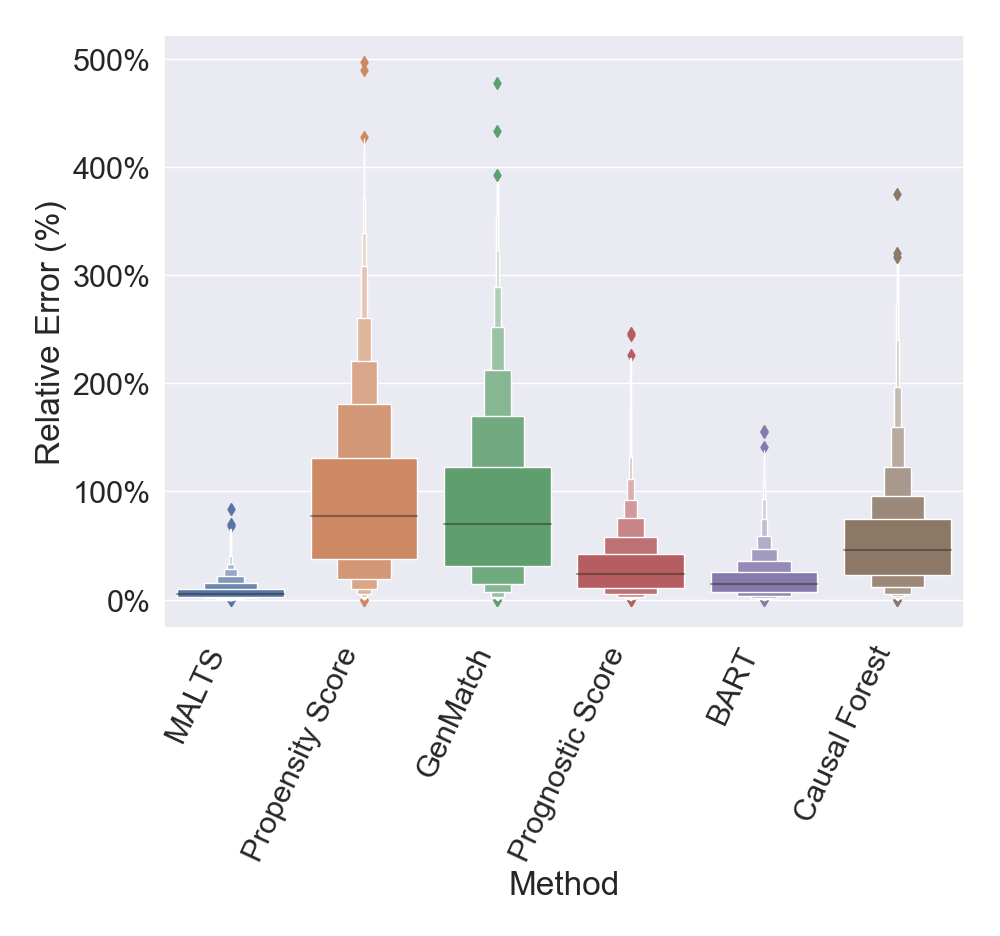
\includegraphics[width=0.7\textwidth]{Figures/boxplot_multifold_malts_continuous.png}    \caption{{\textit{\it MALTS performs well with respect to other methods for continuous data.}} Letter-box plots of CATE Absolute Error on the test set for several methods.}
    \label{fig:continuous}
\end{figure}


% \begin{figure}[h]
%     \centering
%     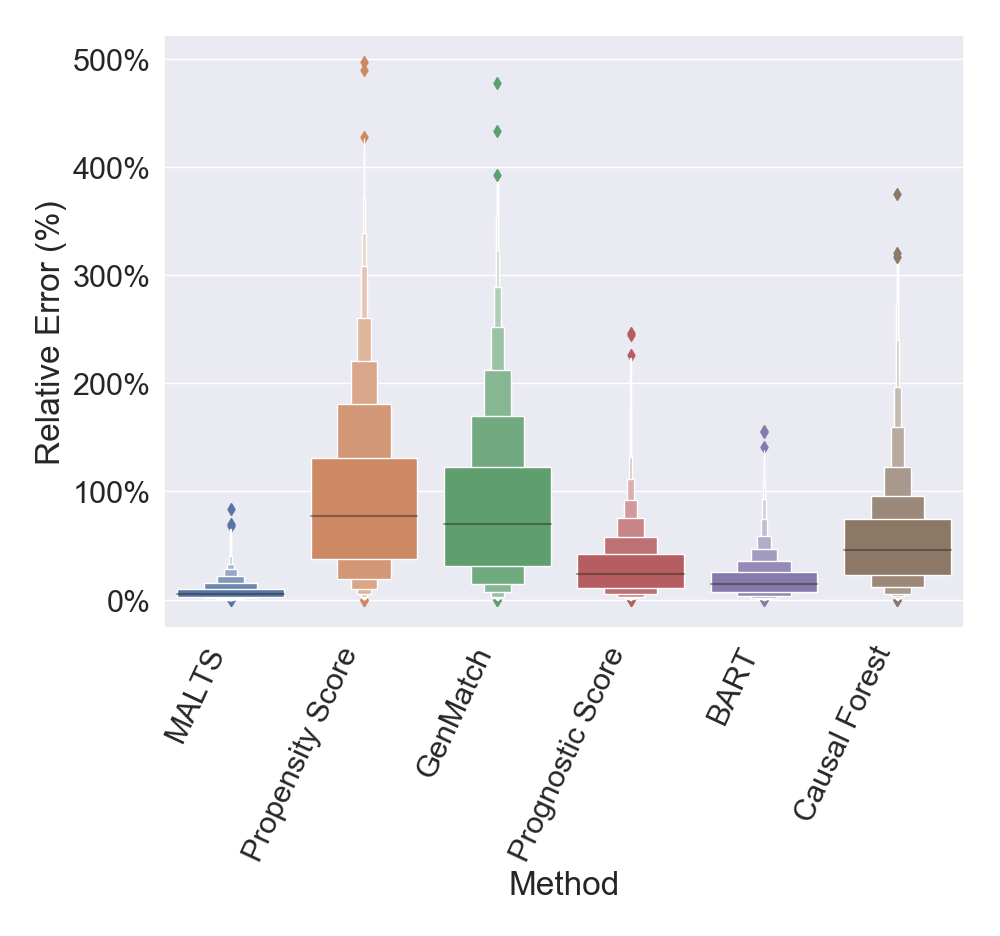
\includegraphics[width=0.85\textwidth]{Figures/boxplot_multifold_malts_continuous.png}\\
%     (a) Continuous Covariates\\
%     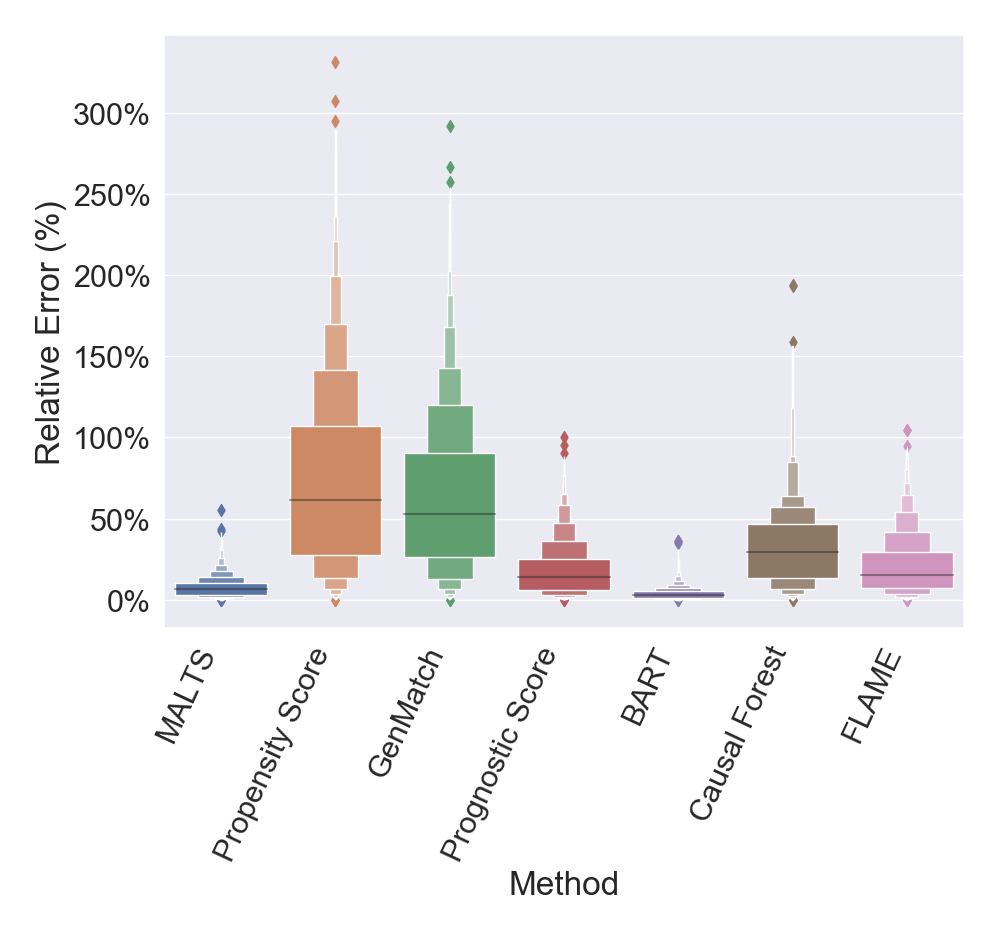
\includegraphics[width=0.9\textwidth]{Figures/boxplot_multifold_malts_discrete.png}\\
%     (b) Discrete Covariates
    
%     \caption{{\textit{\it MALTS performs well with respect to other methods.}} Letter-box plots of CATE Absolute Error on the test set for several methods. MALTS performs well, despite being a matching method, on the setup with (a) continuous covariates, (b) discrete covariates.}
%     \label{fig:continuous}
% \end{figure}

%Figure~\ref{fig:continuous}(a) shows the performance of various causal inference methods on the simulated data. MALTS performance is on par with existing state-of-the-art methods like BART. The error-rate for MALTS is significantly lower compared to prognostic score matching or causal forest.

\subsection{Discrete Covariates}
We use the data-generative process described in Section~\ref{dgp1} to generate 2500 units with no continuous covariates, 15 important discrete covariates and 10 irrelevant discrete covariates. Further, we set the parameters to the DGP as follows:
$\mu = 1$, $\Sigma = 1.5$, $\phi=0.5$, $\sigma = 20$ and $c = 2$. We used the weighted Hamming distance metric for this experiment.
%We compared the CATE estimation error-rates for MALTS in contrast with other existing matching and non-matching methods.

% \begin{figure}
%     \centering
%     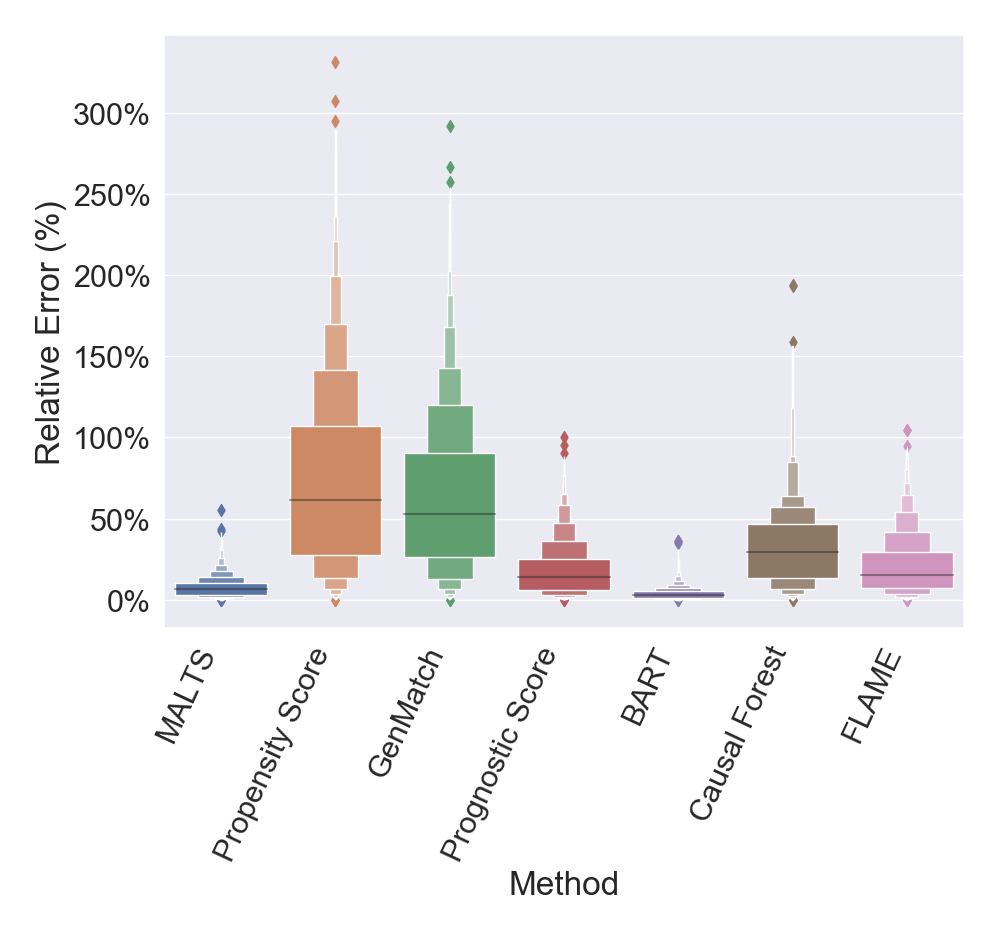
\includegraphics[width=0.9\textwidth]{Figures/boxplot_multifold_malts_discrete.png}
%     \caption{Discrete Covariates}
%     \label{fig:discrete}
% \end{figure}

Figure~\ref{fig:discrete} shows the performance comparison, again showing that 
%of various causal inference methods on the simulated data. 
MALTS' performance is on par with existing state-of-the-art non-matching methods; it also performs better than FLAME (a state-of-the-art matching method for discrete data) as it is able to provide additional smoothing in this relatively small-$n$ setting. \textit{Hence, MALTS performs well for discrete covariates in the quadratic data generation process.}
%methods like BART and the error-rate for MALTS is significantly lower compared to other treatment effect estimation methods prognostic score matching or FLAME.
\begin{figure}
     \centering
    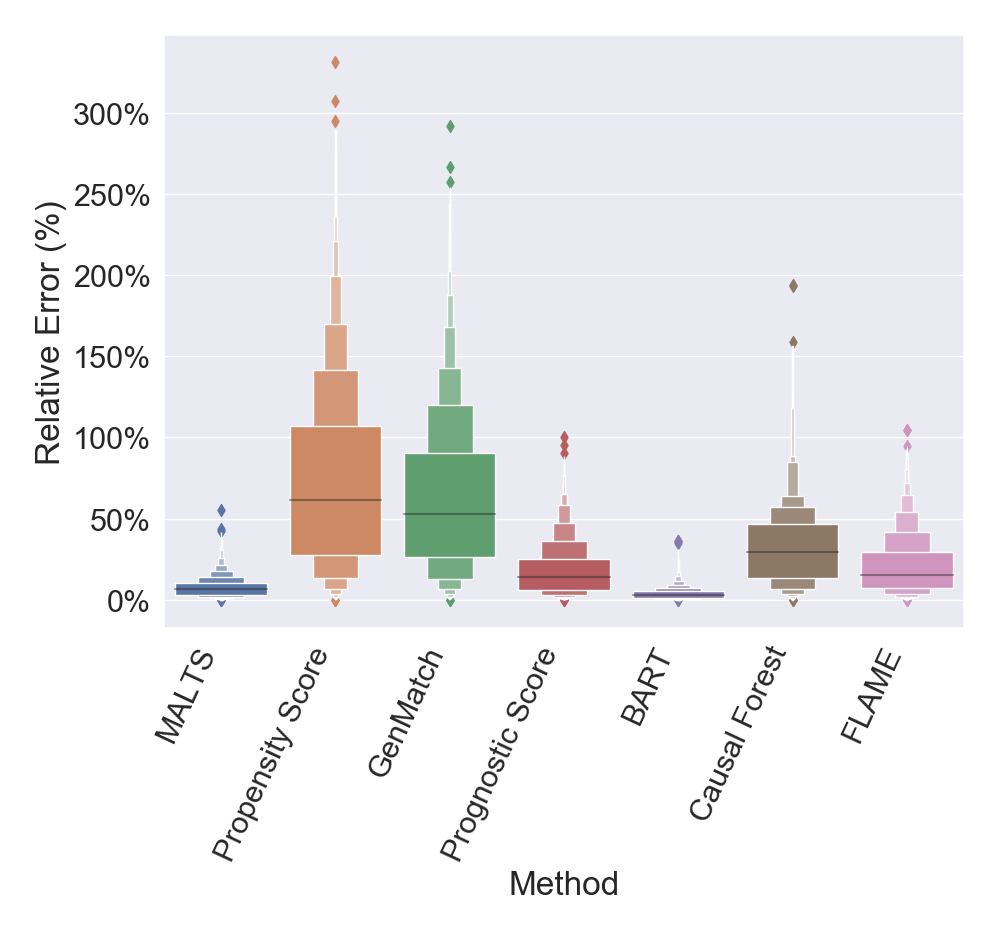
\includegraphics[width=0.65\textwidth]{Figures/boxplot_multifold_malts_discrete.png}    \caption{{\textit{\it MALTS performs well with respect to other methods for discrete data.}} Letter-box plots of CATE Absolute Error on the test set for several methods.}
    \label{fig:discrete}
\end{figure}


\subsection{Mixed Covariates}
We use the data-generative process used for experiments on continous and discrete covariates (described in Section~\ref{dgp1}) to generate 2500 units with 5 relevant continuous covariates, 15 relevant discrete covariates, 10 irrelevant continuous and 10 irrelevant discrete covariates. We used the same set of parameters for the DGP as the previous two experiments. Similarly to the previous two experiments, Figure~\ref{fig:mixed} shows that \textit{MALTS performs on par with the state-of-the-art non-matching methods and outperforms all matching methods that can handle mixed covariates for the quadratic data generation process.}

\begin{figure}[h]
    \centering
    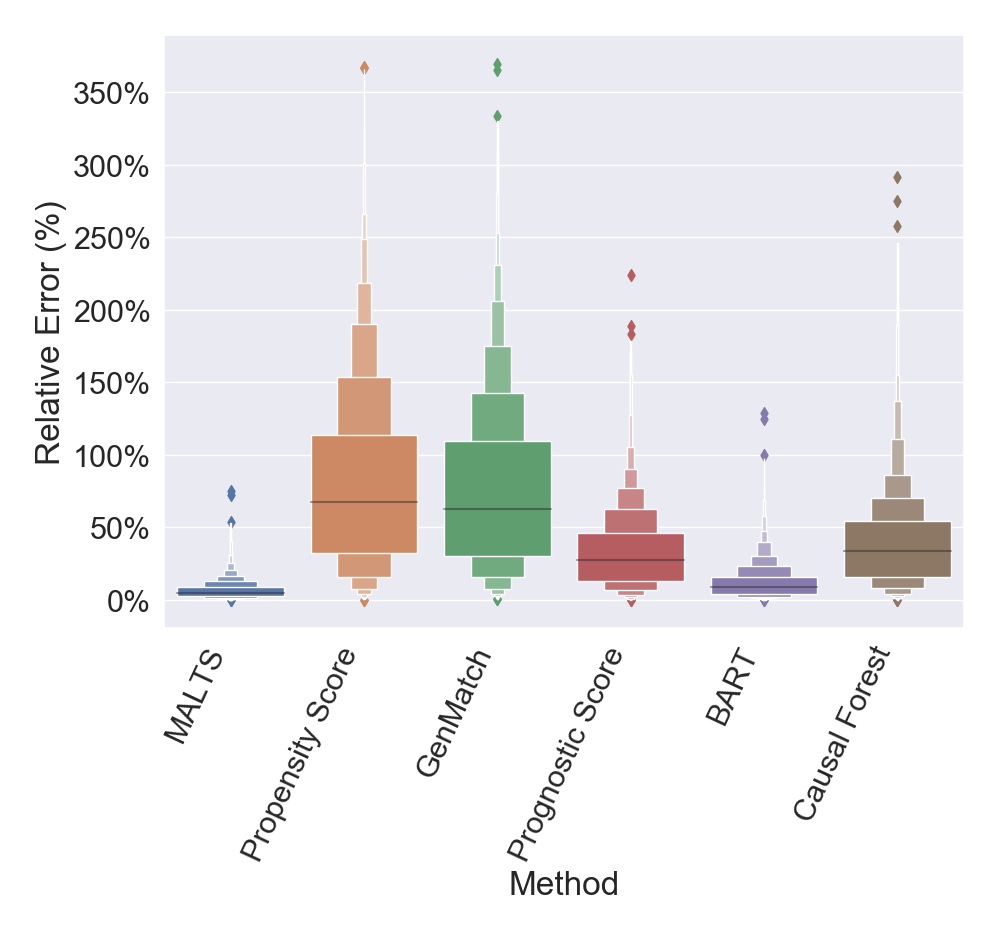
\includegraphics[width=0.65\textwidth]{Figures/boxplot_multifold_malts_mixed.png}
    \caption{{\textit{\it MALTS performs well on data with mixed covariates.}} Letter-box plots of CATE Absolute Error on the test set for several methods. MALTS performs well on the setup with mixed (continuous+discrete) covariates.}
    \label{fig:mixed}
\end{figure}

\subsection{Friedman's Setup}
We further compare MALTS and other flexible methods' performance on data generated using the process described in Section~\ref{dgp2}. 
%We test MALTS and other methods in the DGP mentioned in Section~\ref{dgp2} because the potential outcome functions for the 
This DGP is particularly interesting because the potential outcomes are highly non-linear functions with trigonometric expressions.

\begin{figure}[h]
    \centering
    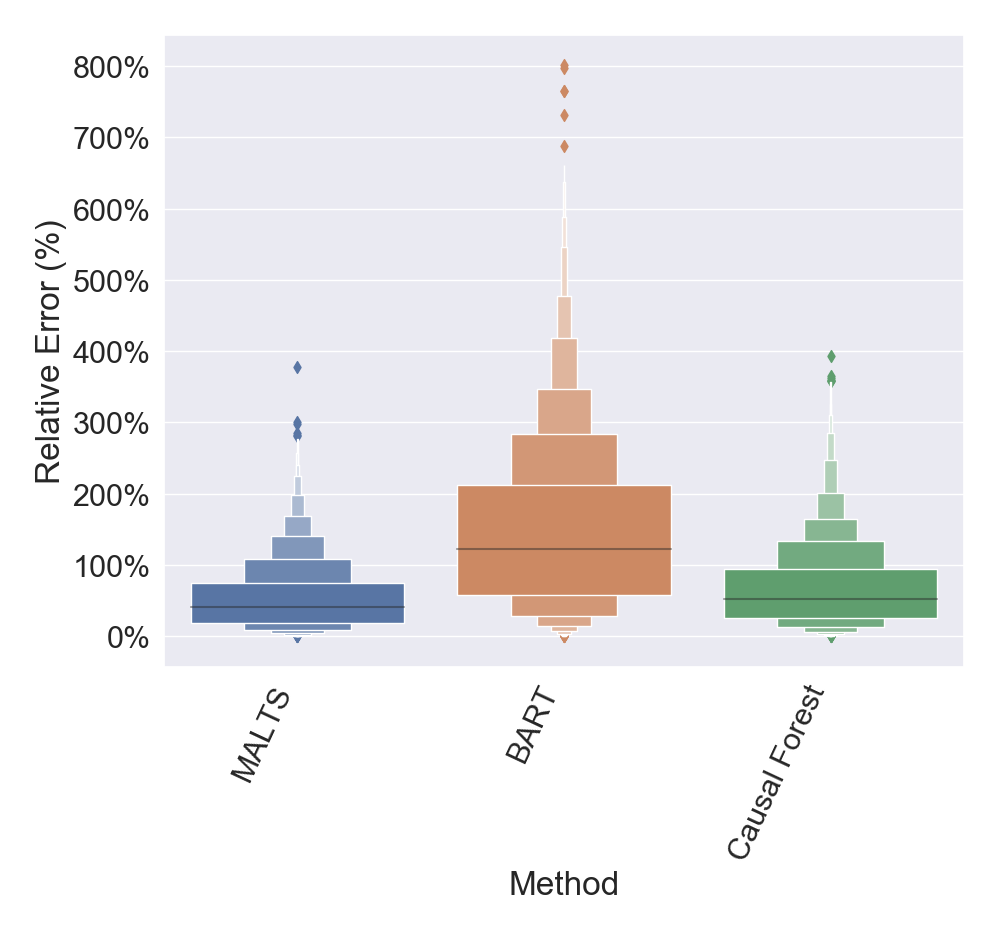
\includegraphics[width=0.65\textwidth]{Figures/boxplot_multifold_malts_friedman_2.png}
    \caption{{\textit{\it MALTS performs well on Friedman's setup.}} Letter-box plots of CATE Absolute Error on the test set for MALTS and two black box methods. 
    %MALTS performs well, despite being a matching method on Friedman's setup with highly non-linear setup with scale trigonometric treatment effect.
    }
    \label{fig:Friedman}
\end{figure}

As shown in Figure~\ref{fig:Friedman}, we observe that \textit{MALTS performs on par with Causal Forest while BART's error-rate is significantly higher (worse) than MALTS, for the Friedman's data generation process}. 

% Based on the experiments comparing the error-rates of various CATE estimation procedures across different simulation setups, MALTS (while being interpretable) also can perform on par or better than the existing methods. 

% We further analyzed MALTS' variance estimates and performance under limited overlap between the covariates' distribution of treated and control groups, shown in Appendix~B. 

%In next subsection, we use MALTS along with other causal inference methods to estimate treatment effect and compare their performance on Lalonde's temporary employment program data.

\subsection{LaLonde Data}
The LaLonde data pertain to the National Support Work Demonstration (NSW) temporary employment program and its effect on income level of the participants \citep{lalonde}. This dataset is frequently used as a benchmark for the performance of methods for observational causal inference. We employ the male sub-sample from the NSW in our analysis as well as the PSID-2 control sample of male household-heads under age 55 who did not classify themselves as retired in 1975 and who were not working when surveyed in the spring of 1976 \citep{dehejia_wahba_nonexp}. The outcome variable for both experimental and observational analyses is earnings in 1978 and the considered variables are age, education, whether a respondent is Black, is Hispanic, is married, has a degree, and their earnings in 1975. Previously, it has been demonstrated that almost any adjustment during the analysis of the experimental and observational variants of these data (both by modeling the outcome and by modeling the treatment variable) can lead to extreme bias in the estimate of average treatment effects \citep{lalonde}.

\begin{table}
 \caption{{\it Predicted ATE for different methods on Lalonde's NSW experimental dataset. The MALTS estimate of ATE is closer to the true ATE than other methods.}}
 \label{tab:lalonde}
 \centering
\begin{tabular}{lrr}
\hline
{} &  \textbf{ATE Estimate} &  \textbf{Estimation Bias (\%)} \\
\textbf{Method}           &               &                      \\
\hline
Truth         &    886 &            - \\
\textit{MALTS}            &    \textit{881.67} &            \textit{-0.49} \\
\textit{MALTS  (pruned)}            &    \textit{888.53} &            \textit{0.29} \\
GenMatch         &    859.72 &            -2.97 \\
Propensity Score &    513.30 &           -42.06 \\
Prognostic Score &    943.81 &             6.52 \\
BART-CV          &   1164.72 &            31.46 \\
Causal Forest-CV &    509.32 &           -42.51 \\
\hline
\end{tabular}
\end{table}

\begin{table}
 \caption{{\it Predicted ATE for different methods on Lalonde's NSW experimental data and PSID-2 observational dataset.} We provide estimates for MALTS before and after pruning the matched groups with large diameters. The threshold to prune was chosen by rule of thumb on diameters of matched groups as shown in Figure~\ref{fig:lalonde_prune}(b).}
 \label{tab:lalonde_psid2}
 \centering
\begin{tabular}{lrr}
\hline
{} &  \textbf{ATE Estimate} &  \textbf{Estimation Bias (\%)} \\
\textbf{Method}          &               &                      \\
\hline
Truth         &    886 &            - \\
\textit{MALTS}            &    \textit{608.37} &             \textit{-31.34} \\
\textit{MALTS (pruned)}            &    \textit{891.75} &             \textit{0.65} \\
GenMatch         &    549.53 &           -37.98 \\
Propensity Score &    513.79 &           -42.01 \\
Prognostic Score &   -897.76 &          -201.33 \\
BART-CV          &    713.20 &           -19.50 \\
Causal Forest-CV &   -179.98 &          -120.31 \\
\hline
\end{tabular}
\end{table}

\textbf{Performance results:} Tables~\ref{tab:lalonde} and \ref{tab:lalonde_psid2} present the average treatment effect estimates based on MALTS, state-of-the-art modeling methods, and matching methods. \textit{MALTS (after appropriately pruning low-quality matched groups) is able to achieve accurate ATE estimation on both experimental and observational datasets.}

Figure~\ref{fig:lalonde_prune} illustrates how the matched groups were pruned. There was a clear visual separation between high-quality matched groups, which had low diameters, and low-quality matched groups, with larger diameters.

%As illustrated in Figure~\ref{fig:lalonde_prune}, the thresholding criteria for the observational Lalonde dataset were determined using the visual observation on diameters of the matched group such that the clusters containing matched groups with large diameters is pruned. 

\begin{figure}
    \centering
    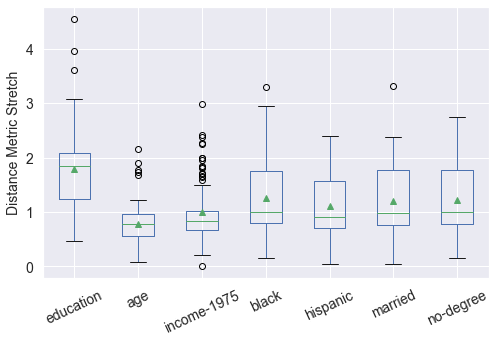
\includegraphics[width=0.75\textwidth]{Figures/m_lalonde.png}\\
    (a) Distance Metric learned on Lalonde data.\\
    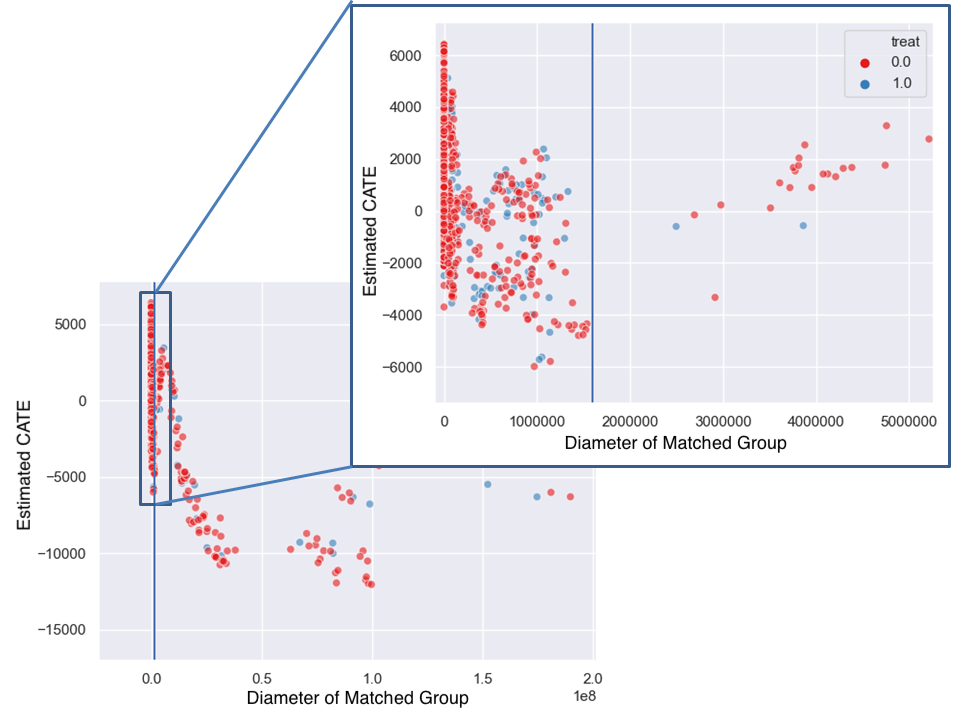
\includegraphics[width=0.9\textwidth]{Figures/lalonde_pruning.png}\\
    (b) Criteria for pruning low-quality matched groups.\\
    \caption{(a) Box-plot of distance metric stretch values corresponding to each covariate in Lalonde data learned over 100 estimations.  (b) Criteria to prune low-quality matched groups with large diameter from Lalonde data.}
    \label{fig:lalonde_prune}
\end{figure}

\textbf{Model Interpretability:}
One difference between MALTS and the other methods is that its solution can be described concisely: MALTS produces a total of seven numbers that define the distance metric. The distribution of the learned distance metric values across folds is shown in Figure~\ref{fig:lalonde_prune}(a). Once the researcher has these seven numbers, along with the value of $k$ in $k$-nearest neighbors used to train MALTS, they know precisely which units should be matched. In contrast, causal forest and BART require a model whose size  depends on the number of trees, where each tree is at least a couple of levels deep--in this case, 2000 trees  and 150 trees, respectively.

\textbf{Interpretability of Matched Groups:}
To examine the interpretability of MALTS' matched groups, we present two of the matched groups from MALTS for the observational Lalonde dataset in Table~\ref{tab:match-group-example}, corresponding to two ``query'' individuals in the dataset.
%We show the learned stretches for the distance metric ($\mathcal{M}$) in Figure~\ref{fig:lalonde_prune}(a). 
 %two individuals for whom we want to construct matched groups:
 Query 1 is a 22 year old with no income in 1975. We are able to construct a tight matched group for this individual (both in control and in treatment). In contrast, Query 2 is a 42-year-old high-income individual without a degree, which is an extremely unlikely scenario, leading to a matched group with a very large diameter, which should probably not be used during analysis. Such granular analysis is not possible for regression methods like BART and matching methods like progostic score or propensity score matching. Table~\ref{tab:mg_prog} in Appendix~D shows an example matched group using prognostic score matching for unit-id-1 (MALTS produces high-quality matched group for this unit as shown in Table~\ref{tab:match-group-example}).

 This further highlights the troubleshooting capabilities of interpretable matching methods: by identifying units that are poorly matched, we know exactly which units to study in more detail. In this case, it is possible that the ``degree'' field might have a data error, which means it would be better not to match this unit and to potentially follow up on the veracity of their responses.

\begin{table}[]
\caption{{\it Learned distance metric and examples of matched-groups on Lalonde Experimental treatment and Observational control datasets for two example query points drawn from the same datasets.} Query 1 represents a high quality (low diameter) matched group while Query 2 represents a poor quality (high diameter) matched group that could be discarded during analysis.}
\label{tab:match-group-example}
\resizebox{\textwidth}{!}{%
\begin{tabular}{rrrrrrrrrr}
\hline
\textbf{} &
  \textbf{} &
  \textbf{Age} &
  \textbf{Education} &
  \textbf{Black} &
  \textbf{Hispanic} &
  \textbf{Married} &
  \textbf{No-Degree} &
  \textbf{Income-1975} &
  \textbf{} \\ \hline
mean($Diag(\mathcal{M})$) & & 0.780 & 1.786 & 1.254 & 1.110 & 1.205 & 1.229 & 1.001 &  \\
std($Diag(\mathcal{M})$) & & 0.361 & 0.778 & 0.641 & 0.577 & 0.614 & 0.618 & 0.512 &  \\ \hline
\end{tabular}%
}
\vskip 5mm
\resizebox{\textwidth}{!}{%
\begin{tabular}{lrrrrrrrrr}
\hline
\textbf{Unit-id} &
  \textbf{Treated} &
  \textbf{Age} &
  \textbf{Education} &
  \textbf{Black} &
  \textbf{Hispanic} &
  \textbf{Married} &
  \textbf{No-Degree} &
  \textbf{Income-1975} &
  \textbf{Income-1978} \\ \hline
Query-1: \textit{1}   & 1.0 & 22.0 & 9.0  & 0.0 & 1.0 & 0.0 & 1.0 & 0.0 & 3595.89  \\  \hline
\textit{94}  & 1.0 & 23.0 & 8.0  & 0.0 & 1.0 & 0.0 & 1.0 & 0.0 & 3881.28  \\
\textit{330} & 0.0 & 22.0 & 8.0  & 0.0 & 1.0 & 0.0 & 1.0 & 0.0 & 9920.94  \\
\textit{299} & 0.0 & 22.0 & 9.0  & 1.0 & 0.0 & 0.0 & 1.0 & 0.0 & 0.00     \\
\textit{5}   & 1.0 & 22.0 & 9.0  & 1.0 & 0.0 & 0.0 & 1.0 & 0.0 & 4056.49  \\
\textit{82}  & 1.0 & 21.0 & 9.0  & 1.0 & 0.0 & 0.0 & 1.0 & 0.0 & 0.00     \\
\textit{416} & 0.0 & 22.0 & 9.0  & 1.0 & 0.0 & 0.0 & 1.0 & 0.0 & 12898.38 \\
\textit{333} & 0.0 & 21.0 & 9.0  & 1.0 & 0.0 & 0.0 & 1.0 & 0.0 & 3343.22  \\
\textit{292} & 1.0 & 20.0 & 9.0  & 1.0 & 0.0 & 0.0 & 1.0 & 0.0 & 8881.67  \\
\textit{17}  & 1.0 & 23.0 & 10.0 & 1.0 & 0.0 & 0.0 & 1.0 & 0.0 & 7693.40  \\
\textit{116} & 1.0 & 24.0 & 10.0 & 1.0 & 0.0 & 0.0 & 1.0 & 0.0 & 0.00     \\ \hline
\end{tabular}%
}
\vskip 5mm
\resizebox{\textwidth}{!}{%
\begin{tabular}{lrrrrrrrrr}
\hline
\textbf{Unit-id} &
  \textbf{Treated} &
  \textbf{Age} &
  \textbf{Education} &
  \textbf{Black} &
  \textbf{Hispanic} &
  \textbf{Married} &
  \textbf{No-Degree} &
  \textbf{Income-1975} &
  \textbf{Income-1978} \\
\hline
Query-2: \textit{968} &    0.0 &  42.0 &       11.0 &    0.0 &       0.0 &      1.0 &       1.0 &  44758.07 &  54675.88 \\
\hline
\textit{274} &    1.0 &  35.0 &        9.0 &    1.0 &       0.0 &      1.0 &       1.0 &  13830.64 &  12803.97 \\
\textit{141} &    1.0 &  25.0 &        8.0 &    1.0 &       0.0 &      0.0 &       1.0 &  37431.66 &   2346.83 \\
\textit{967} &    0.0 &  50.0 &       17.0 &    0.0 &       0.0 &      1.0 &       0.0 &  30435.48 &  25860.21 \\
\textit{948} &    0.0 &  35.0 &       12.0 &    0.0 &       0.0 &      1.0 &       0.0 &  26854.84 &  29554.53 \\
\textit{210} &    1.0 &  25.0 &        8.0 &    0.0 &       0.0 &      0.0 &       1.0 &  23096.65 &   6421.53 \\
\textit{241} &    1.0 &  24.0 &       15.0 &    1.0 &       0.0 &      0.0 &       0.0 &  13008.50 &  14683.63 \\
\textit{311} &    0.0 &  28.0 &       12.0 &    1.0 &       0.0 &      1.0 &       0.0 &  29009.11 &  10067.43 \\
\textit{183} &    1.0 &  23.0 &       10.0 &    1.0 &       0.0 &      0.0 &       1.0 &  15709.56 &   5665.07 \\
\textit{182} &    1.0 &  23.0 &       12.0 &    1.0 &       0.0 &      1.0 &       0.0 &  15079.95 &  10283.49 \\
\hline
\end{tabular}
%
}
\end{table}